% Created with jtex v.1.0.20
\documentclass{article}
\PassOptionsToPackage{short, nodayofweek}{datetime}


% Start Curvenote Definitions

% Pass Options Section
% base
\PassOptionsToPackage{normalem}{ulem}
\PassOptionsToPackage{utf8}{inputenc}

% template
\PassOptionsToPackage{framemethod=TikZ}{mdframed}
\PassOptionsToPackage{x11names, svgnames}{xcolor}

%%% PACKAGES

% base
\usepackage{inputenc}
\usepackage{url}
\usepackage{graphicx}
\usepackage{adjustbox}
\usepackage{amssymb}
\usepackage{amsfonts}
\usepackage{amsmath}
\usepackage{enumitem}
\usepackage{nicefrac}
\usepackage{booktabs}
\usepackage{microtype}
\usepackage{hyperref}
\usepackage{ulem}
\usepackage{enumitem}
\usepackage{float}
\usepackage{datetime}
\usepackage{xkeyval}
\usepackage{framed}
\usepackage{doi}

% template
\usepackage{natbib}
\usepackage{fancyvrb}
\usepackage{mdframed}
\usepackage{xcolor}

%%%


%%%% Setup Section

% base
\graphicspath{{.}}
% template
\sloppy
\newenvironment{aside}{\begin{framed}}{\end{framed}}
\newmdenv[linewidth=2pt,linecolor=CornflowerBlue,topline=false,bottomline=false,rightline=false,leftline=true,skipabove=20,skipbelow=20,leftmargin=20,rightmargin=20]{callout}
\newfloat{code}{thp}{loc}
\floatname{code}{Program}
\raggedbottom
\bibliographystyle{abbrvnat}
\setcitestyle{authoryear,open={(},close={)},semicolon,aysep={,}}

% End Curvenote Definitions




% colors for hyperlinks
\hypersetup{colorlinks=true, allcolors=blue}
\hypersetup{
pdftitle={\@title},
pdfsubject={},
pdfauthor={\@author},
pdfkeywords={},
addtopdfcreator={Written in Curvenote}
}

\usepackage{curvenote}

\title{Ch. 10: Instrumentation of a simple myoelectric prosthetic}

\newdate{articleDate}{24}{2}{2025}
\date{\displaydate{articleDate}}

\author{\bfseries Erin McKiernan\mdseries\\Universidad Nacional Autónoma de México (UNAM), Open Research Community Accelerator (ORCA)\\\AND\bfseries Daniel Gómez Pérez\mdseries\\}

\begin{document}

\maketitle
\keywords{}

\section{Overview}

In this laboratory practical, students will learn about the basic anatomy of the hand, and how the muscles and tendons of the hand work together to control its movement. Students will learn how to build a simple prosthetic hand from lightweight materials, how to connect this hand to a programmable interface, and how to control movement of the hand by feeding electromyographics signals from the bicep muscle through the interface. Overall, this practical will help students to better understand the biomechanics of one part of the musculoskeletal system, the instrumentation of simple prosthetics, and the relationship between electrical signals and movement. This practical could be carried out in multiple class sessions of variable durations, as students work to build the model hand, program the interface, and test it. Or, this could be done asynchronously as an assigned project. While not necessary, it is recommended that students carry out the experimental practical in \href{https://curvenote.com/oxa:EPpXta8zJdzN048lz8AR/hZTnTYzQR5EQmCKX51Wj}{Ch. 1: Muscle physiology and EMG basics }prior to this practical.

\section{Learning objectives}

\textbf{Before} doing this lab, students should be able to:

\begin{itemize}
\item describe the structure and function of the main elements of the musculoskeletal system, including bones, joints, muscles, ligaments, and tendons
\item explain the mechanisms of muscle contraction and force generation
\item understand the basics of electromyography (EMG) recording
\end{itemize}

\textbf{During} this lab, students will:

\begin{itemize}
\item explore the basic anatomy of the hand, including the key muscles and tendons and how to represent these in the construction of a model hand
\item investigate the biomechanics of hand and finger movements
\item learn about Arduino programming and how to control a servomotor
\end{itemize}

\textbf{After} doing this lab, students should be able to:

\begin{itemize}
\item describe the basic concepts underlying myoelectric prosthestic instrumentation
\item generate ideas to improve the prosthetic design
\end{itemize}

\section{Equipment and materials}

\begin{itemize}
\item \href{https://docs.backyardbrains.com/retired/products/musclespikershieldbundle}{Muscle SpikerShield} (Backyard Brains)
\item 9V battery with leash cable (to power, if no other power source connected)
\item Round surface electrodes (any medical supply provider)
\item Cable with alligator clips to connect electrodes to SpikerBox (Backyard Brains)
\item Cable to connect SpikerBox to a laptop computer (Backyard Brains)
\item Computer with open-source \href{https://docs.arduino.cc/software}{Arduino software} installed
\item Alcohol and cotton swabs to help remove electrodes after recording (optional)
\item Cardboard, or other lightweight material, that can be cut into shape and is flexible
\item Heavy-duty threads, each approximately 30 cm long (x5)
\item Glue, tape, or staples and stapler (depending on preferred method for fixing threads)
\item Silicon glue and glue gun
\item Servomotor (MG995, or similar model)
\item Other indications: Wear loose clothing to permit electrode placement
\end{itemize}

\section{Background}

\subsection{Limb loss and myoelectric prostheses}

Every year, thousands of people worldwide undergo amputation of limbs due to trauma, vascular complications, and disease, among other causes. A 2008 study estimated that, as of 2005, around 1.6 million people in the U.S. were living with limb loss, of which over 500,000 were designated as loss of an upper limb including hands and fingers \citep{ziegler2008estimating}. Those numbers were projected to double by the year 2050. A more recent 2024 study estimated that the total in the U.S was now over 2.3 million, saying this number would double by 2050 and increase 145\% by 2060 \citep{rivera2024estimating}.

For those living with limb loss, a prosthesis (artificial limb) can help them to regain function and independence. There exist different types of prostheses, ranging from simply aesthetic to varying degrees of functionality \citep{maat2018passive, ten20173d}. Some of the most promising are myoelectric prostheses, which use electromyogram (EMG) signals recorded from skeletal muscles to control movements of the artificial limb \citep{geethanjali2016myoelectric, iqbal2018review, igual2019myoelectric}. While the idea for these devices was first proposed in the late 1940s, huge leaps have been made in recent years due to advances in areas like sensor technology and machine learning. In general, such devices include: (1) a \textbf{detection} step, during which the EMG signal is recorded, (2) a \textbf{processing} step, during which certain features of the EMG signal are measured, extracted, or classified, and (3) a \textbf{control} step, during which these features are fed into a digital interface that is programmed to respond in prescribed ways to then send commands to the prosthetic limb. What often varies between different models is the complexity of the signal processing and the control mechanisms (reviewed in \citet{geethanjali2016myoelectric}). The simple device we will build is based on a \href{http://single.channel}{single.channel} EMG with amplitude measurement fed into a servomotor. A more complex scheme can be seen in Figure~\ref{w1uHQcGVm9}.

\begin{figure}[!htbp]
\centering
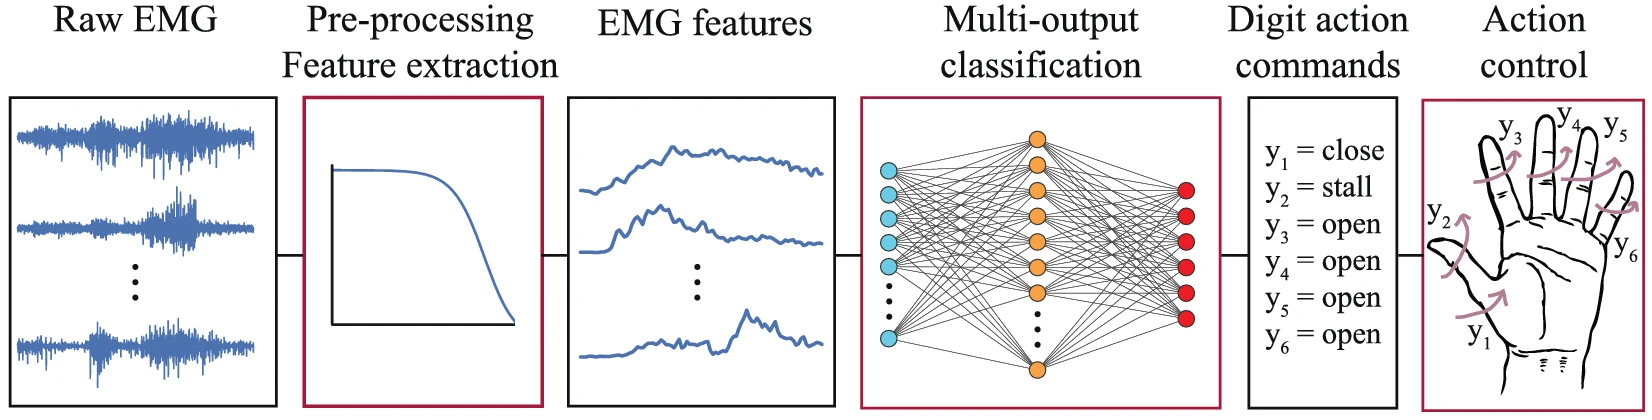
\includegraphics[width=1\linewidth]{files/EPpXta8zJdzN048lz8AR-b0dec1aab40cc143e6fe874233a554f2.png}
\caption[]{``Action decoding paradigm'' based on multi-channel EMG recordings used to control the digits of a prosthetic hand. Image credit: Krasoulis, A., Nazarpour, K. \textit{Sci Rep} \textbf{10}, 16872 (2020). \cite{Krasoulis_2020}, CC BY.}
\label{w1uHQcGVm9}
\end{figure}

\subsubsection{Servomotors}

Myoelectric prosthetics require a motor to achieve movement of the artificial limb, and many designs use servomotors (`servos') \citep{ten20173d}. According to \textit{A Dictionary of Mechanical Engineering}, a servomechanism is ``a control system for the position and time derivatives (for example, velocity) of a mechanical system using closed-loop control'', and a servomotor is ``a rotational or translational motor\dotswhich serves to apply torque or force to a mechanical system'' \citep{escudier2019dictionary}. Servos have a number of advantages over other motor types, including their relatively small size, low cost, high speed, and precision control \citep{bbclaw, ellis2012basics}.

Typically, servos have three cables, namely power, ground, and pulse (note the colors, as we will use these to connect the right cables to the right ports on the control board, see Section~\ref{nK7MnuzzrL}). The first two are self-explanatory given their names, while the last (pulse) refers to the cable that connects to the microcontroller (e.g. Arduino) generating the stimulus signal \citep{bbclaw}. Many servos are controlled using Pulse Width Modulation (PWM). In a PWM system, a square-wave pulse is produced, and the duration (width) of the pulse determines how far the motor will rotate, i.e. the angle \citep{}Figure \%s ``. Longer durations mean larger angles. In our model, the degree of rotation will determine the pull on the thread `tendons' and thus how much the model hand closes.

\begin{figure}[!htbp]
\centering
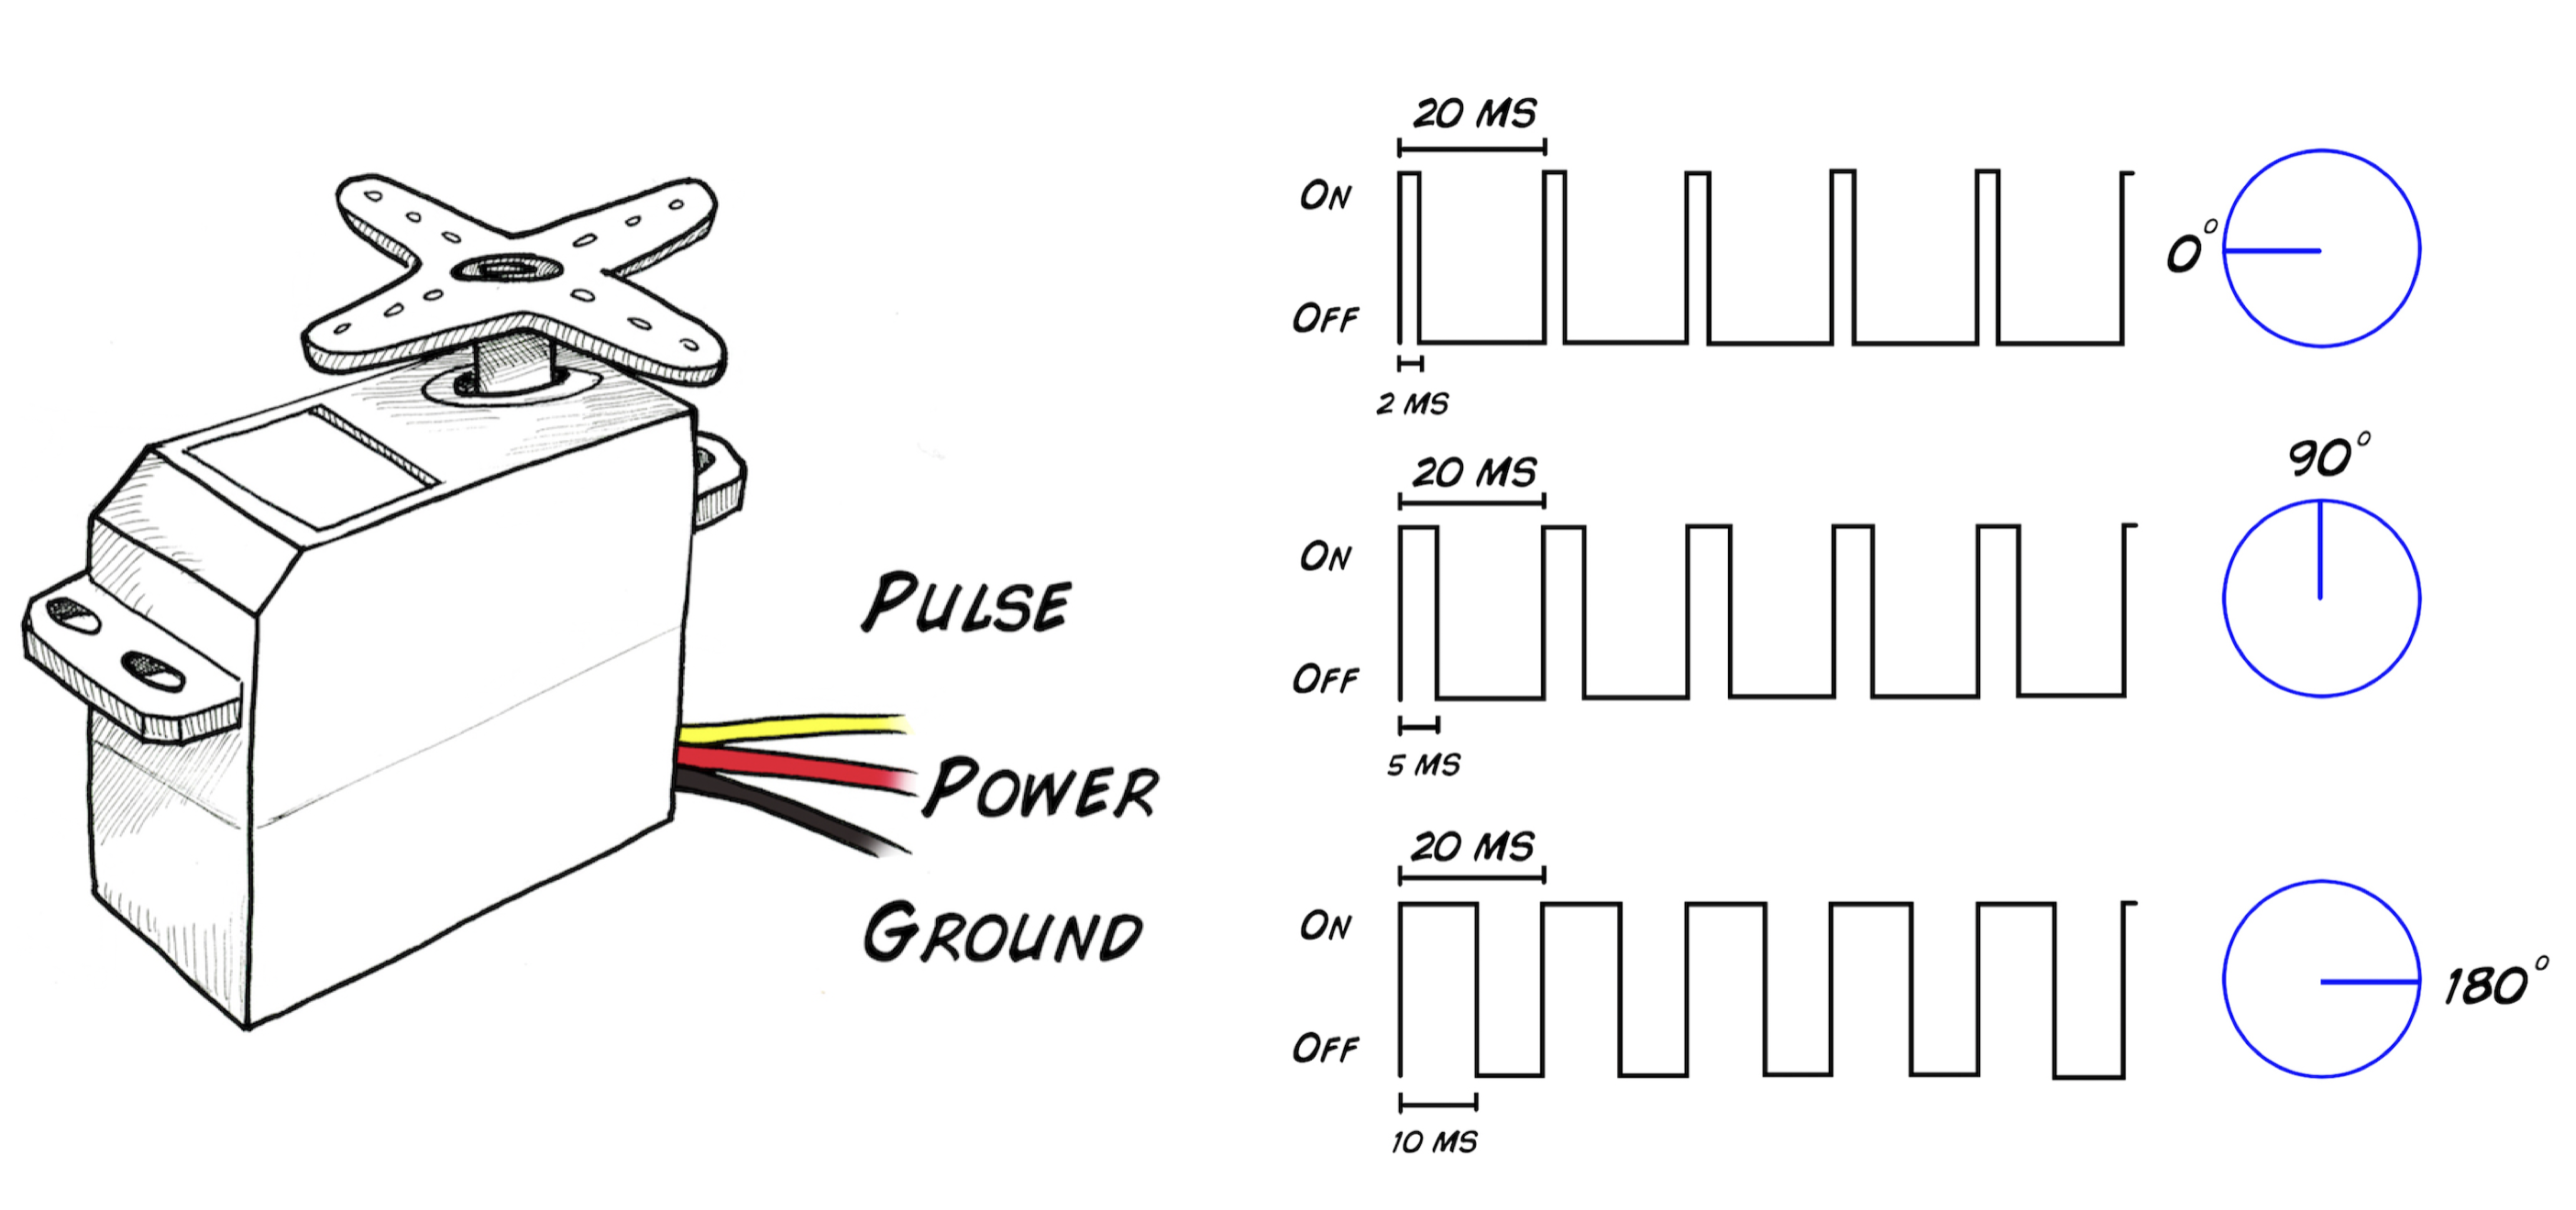
\includegraphics[width=0.9\linewidth]{files/EPpXta8zJdzN048lz8AR-668fb5e878304ce5b48e2ee40f6cd3a6.png}
\caption[]{Servomotor and PWM (Pulse Width Modulation). Image credit: Backyard Brains, \href{https://docs.backyardbrains.com/retired/experiments/MuscleSpikerShield\_GripperHand}{https://docs.backyardbrains.com/retired/experiments/MuscleSpikerShield\_GripperHand}}
\label{SUpFkoFTj4}
\end{figure}

\subsection{Bones and joints of the human hand}

If we want to model the human hand, it is necessary to first know its anatomy. The human hand has a complex skeletal structure, comprising 27 individual bones \citep{panchal2013skeletal} (Fig. 1). Starting proximally, at the base of the hand, we have the 8 carpal bones which make up the wrist. Morphologically, the carpal bones are classified as short bones, with cuboid-like appearance \citep{openStax_bones}. Short bones allow for some movement, but are more for structural support. Moving distally, we find the 5 metacarpal bones, which run through the palm area of the hand. Metacarpal bones are classified as long bones, and their primary function is to connect the wrist to the fingers. More distally still, we have the 14 phalanges, also classified as long bones and divided into the proximal, intermediate, and distal phalanges. Note that the thumb is the only digit which does not have an intermediate phalanx. Articulations of the different phalanges allow for gross motor movements such as grasping, as well as fine motor movements like playing the piano or threading a needle \citep{duncan2013biomechanics}.

\begin{figure}[!htbp]
\centering
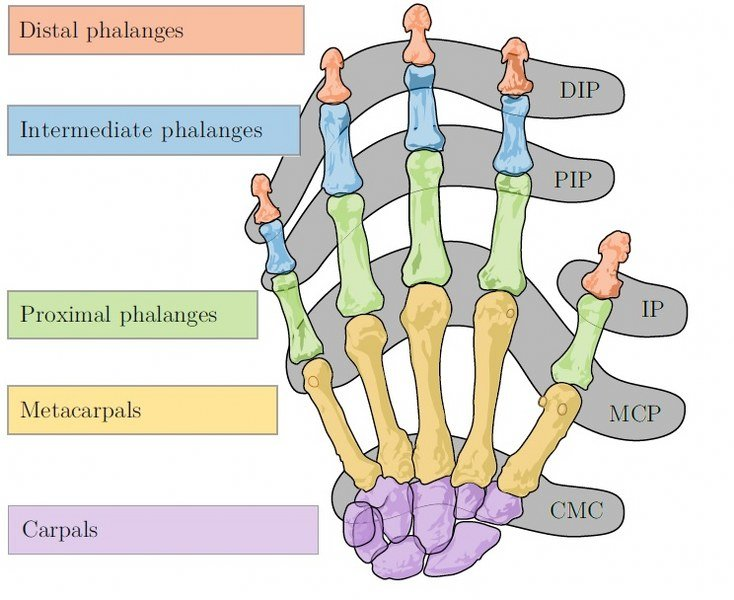
\includegraphics[width=0.6\linewidth]{files/EPpXta8zJdzN048lz8AR-c0f7102765d12d6a28f615efc2b5b74d.png}
\caption[]{Bones and joints in the human hand. Image credit: Tavakoli, Batista, Sgrigna (2015) \cite{Tavakoli_2015}}
\label{Q9rw6fWrIJ}
\end{figure}

Joints form where the different bones in the hand meet \citep{tortora2018principles} (Fig. 1). The meeting points between the carpal and metacarpal bones are called the carpometacarpal (CMC) joints \citep{panchal2013skeletal, ombregt2013applied}. These joints allow for movements like flexion, extension, and rotation of the hand. Where the proximal metacarpals and phalanges meet are known as the metacarpophalangeal (MCP) joints. The proximal interphalangeal (PIP) joints are where the proximal and intermediate phalanges meet. These joints allow you to bend (flex) your fingers at their midpoint. Both the MCP and PIP joints are important in actions such as forming a fist and gripping, and also participate in fine motor movements \citep{duncan2013biomechanics}. Finally, where the intermediate and distal phalanges meet are the distal interphalangeal (DIP) joints. The DIP joints have much more restricted movement compared to the MCP and PIP joints, but do allow some flexion. Note that because the thumb lacks an intermediate phalanx \citep{panchal2013skeletal}, it only has an interphalangeal (IP) joint where the proximal and distal phalanges meet (Fig. 1).

\subsection{Muscles of the human hand}

The force required to move the bones of the hand is provided by skeletal muscles. These muscles can be divided into two main groups, those intrinsic and those extrinsic to the hand \citep{tortora2018principles, ombregt2013applied, openStax_upper}.

\subsubsection{Intrinsic muscles of the hand}

The intrinic muscles both arise from and terminate in the hand \citep{tortora2018principles, ombregt2013applied, schreuders2007intrinsic, openStax_upper} (Fig. 2). They are classified into groups based on anatomical location and function.

Thenar muscles:

\begin{itemize}
\item \textit{abductor pollicis brevis}: abduction of the thumb (first digit) at the CMC joint, moving it away

from the palm at a 90\textsuperscript{o} angle; participates in opposition and flexion of the thumb


\item \textit{adductor pollicis}: adduction of the thumb at the CMC joint, moving it back towards the palm


\item \textit{opponens pollicis}: flexion of the thumb at the CMC joint to produce opposition, where the

thumb comes into contact with the other fingers


\item \textit{flexor pollicis brevis}: flexion of the thumb at the MCP joint
\end{itemize}

Hypothenar muscles:

\begin{itemize}
\item \textit{abductor digiti minimi}: abduction of the little finger (fifth digit) at the MCP joint, moving it

away from the ring finger (fourth digit)


\item \textit{flexor digiti minimi brevis}: flexion of the little finger at the MCP joint


\item \textit{opponens digiti minimi}: flexion and rotation of the little finger at the CMC joint to bring it into

contact (opposition) with the thumb
\end{itemize}

Interosseous muscles:

\begin{itemize}
\item \textit{dorsal interossei}: abduction of the digits, spreading the fingers out and away from the midline;

participate in flexion of the MCP joints and extension of the PIP and DIP joints


\item \textit{palmar interossei}: adduction of the digits, bringing the fingers toward the midline; participate

in flexion of the MCP joints and extension of the PIP and DIP joints
\end{itemize}

Lumbricalis muscles:

\begin{itemize}
\item \textit{I, II, III, IV}: together with the interosseous muscles, all four muscles participate in flexion of

the MCP joints and extension of the IP joints of the 2nd through 5th digits, respectively
\end{itemize}

\begin{figure}[!htbp]
\centering
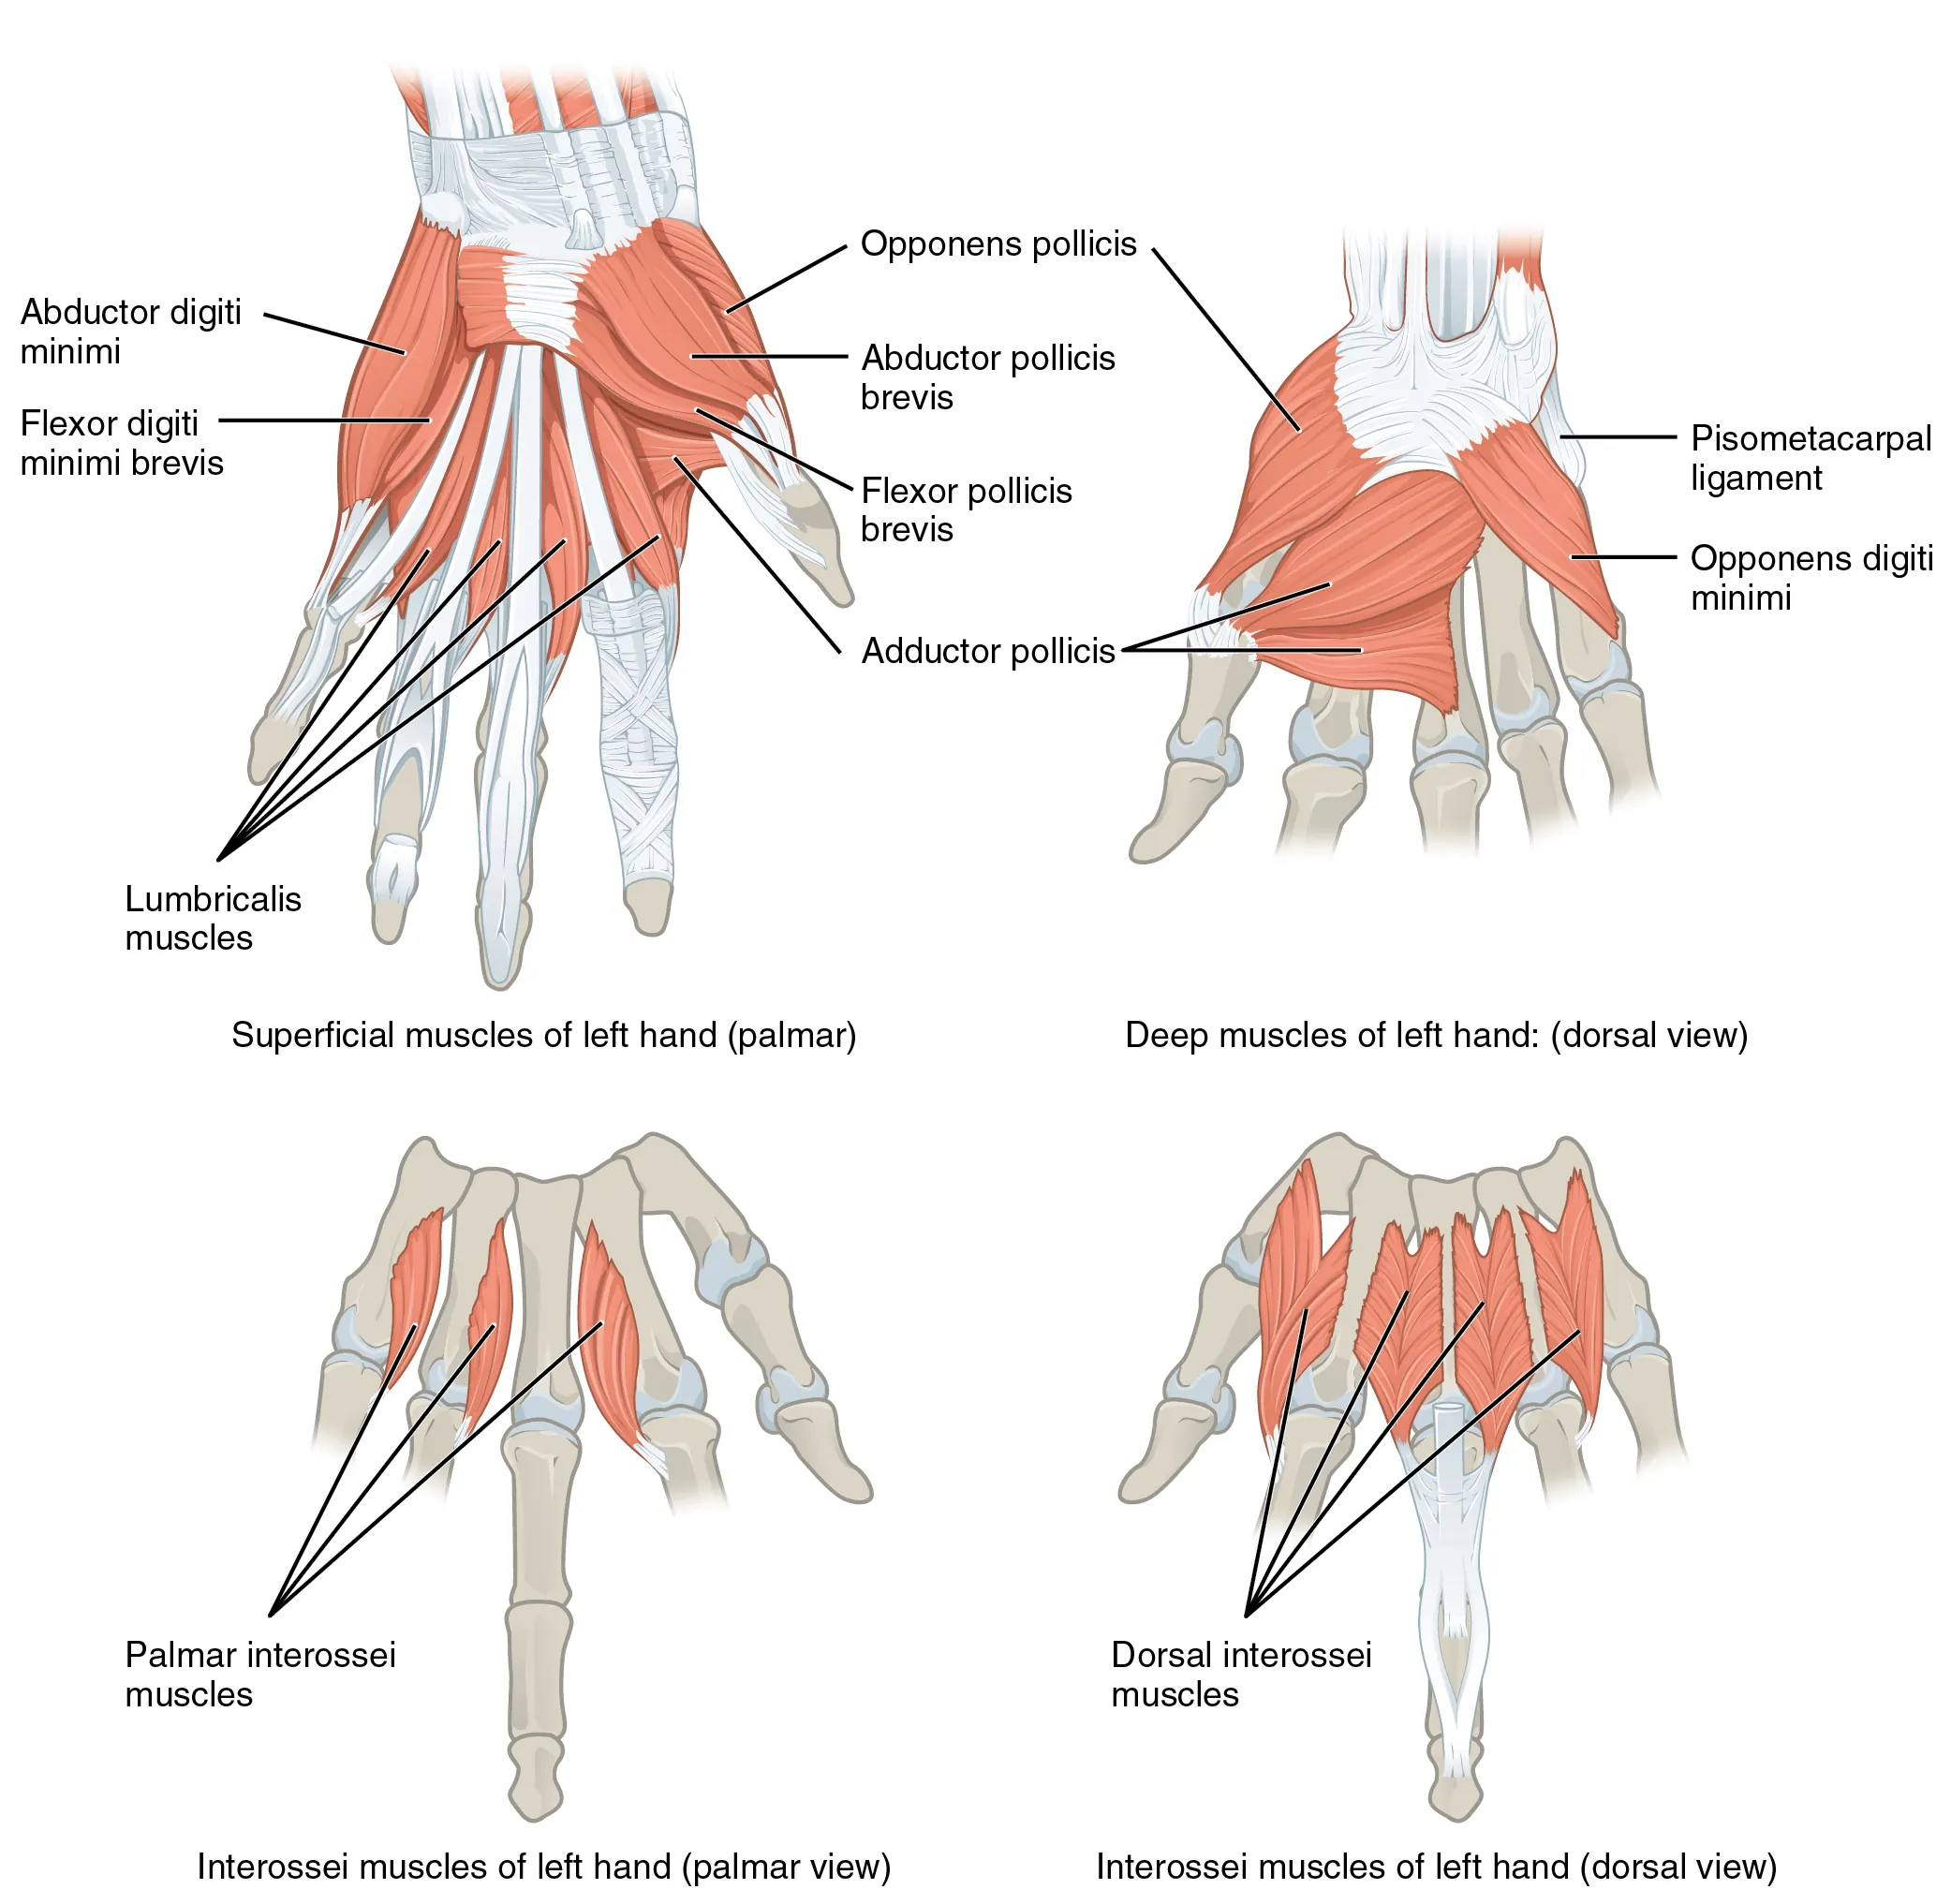
\includegraphics[width=0.7\linewidth]{files/EPpXta8zJdzN048lz8AR-d87e80f99dcfe8a7d01e23b64ddf702a.png}
\caption[]{Intrinsic muscles of the hand. Image credit: OpenStax \href{https://openstax.org/books/anatomy-and-physiology-2e/pages/11-5-muscles-of-the-pectoral-girdle-and-upper-limbs}{https://openstax.org/books/anatomy-and-physiology-2e/pages/11-5-muscles-of-the-pectoral-girdle-and-upper-limbs}}
\label{s5tQEqPmlm}
\end{figure}

\subsubsection{External muscles of the hand}

The external muscles are those which originate outside the hand, primarily in the forearm, but insert into the hand \citep{tortora2018principles, ombregt2013applied, openStax_upper} (Fig. 3).

The extrinsic flexors include:

\begin{itemize}
\item \textit{flexor carpi ulnaris}: flexion and adduction of the hand at the wrist


\item \textit{palmaris longus}: aids in flexion of the hand at the wrist


\item \textit{flexor carpi radialis}: flexion and abduction of the hand at the wrist


\item \textit{flexor digitorum superficialis}: flexion of the 2nd to 5th digits at the PIP and MCP joints (after

flexion is initiated)


\item \textit{flexor digitorum profundus}: flexion of the 2nd to 5th digits at the DIP, PIP, and MCP joints

(after flexion is initiated)


\item \textit{flexor pollicis longus}: flexion of the thumb at the IP and MCP joints
\end{itemize}

The extrinsic extensors include:

\begin{itemize}
\item \textit{extensor carpi radialis longus}: extension and abduction of the hand at the wrist
\item \textit{extensor carpi radialis brevis}: extension and abduction of the hand at the wrist
\item \textit{extensor digitorum}: extension of 2nd to 5th digits at the MCP and IP joints; wrist extension
\item \textit{extensor digiti minimi}: extension of the little finger (5th digit) at the MCP and PIP joints
\item \textit{extensor carpi ulnaris}: extends and adducts the hand at the wrist
\item \textit{abductor pollicis longus}: abduction of the thumb and extension at the CMC joint
\item \textit{extensor pollicis brevis}: extension of the thumb at the MCP joint
\item \textit{extensor pollicis longus}: extension of the thumb at the CMC and IP joints
\item \textit{extensor indicis}: extension of the index finger (2nd digit) at all joints
\end{itemize}

\begin{figure}[!htbp]
\centering
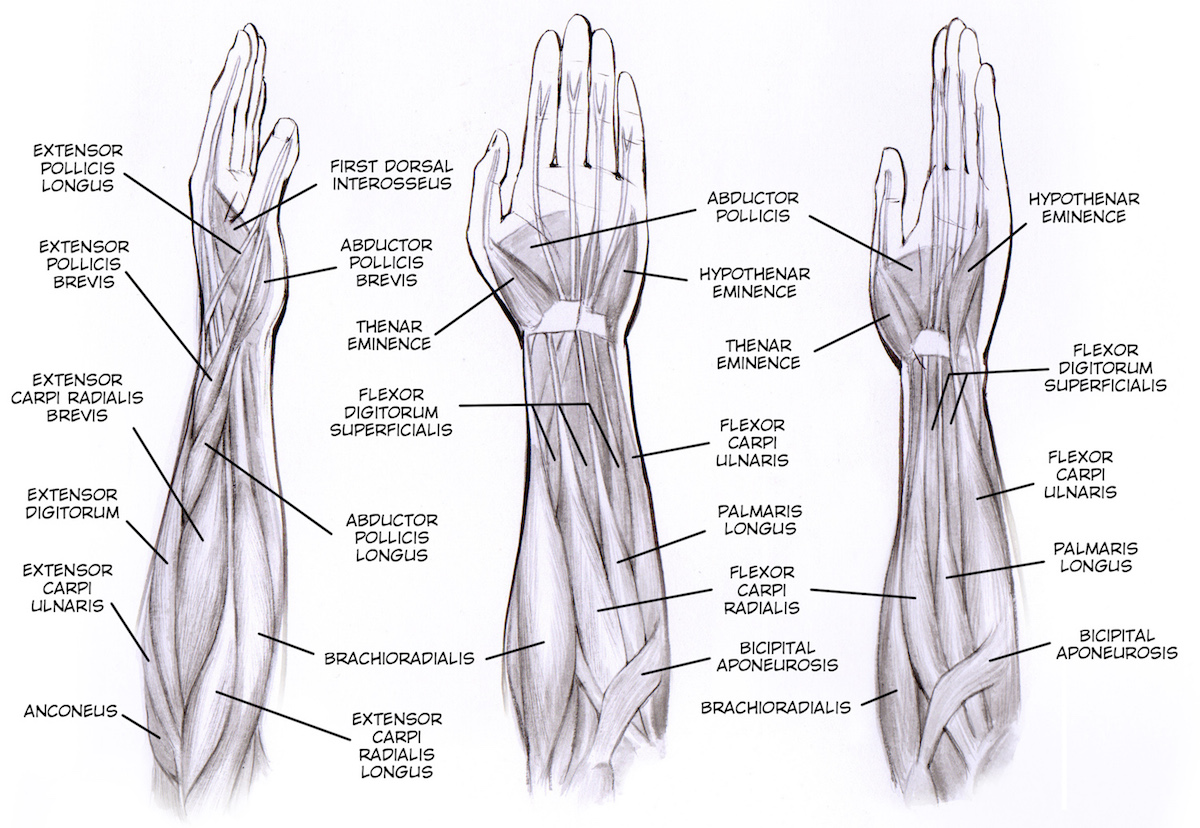
\includegraphics[width=0.7\linewidth]{files/EPpXta8zJdzN048lz8AR-7a67f58c3616b210fcf078d1714aa2fb.png}
\caption[]{Some of the intrinsic and extrinsic muscles of the hand. Image credit: Backyard Brains \href{https://docs.backyardbrains.com/retired/experiments/RobotHand/}{https://docs.backyardbrains.com/retired/experiments/RobotHand/}}
\label{f1XadeuWyO}
\end{figure}

\subsection{Tendons of the hand}

Tendons are collagenous fibers that connect muscles to bone \citep{tortora2018principles}. When a muscle contraction occurs, the force generated is transmitted to the bones via the tendons \citep{kirkendall1997function}. We can think of these tendons like cords; depending on where the cords insert, pulling on them will produce movement at different joints. Since they extend from the muscle, the corresponding tendons bear the same name as the muscle itself. Therefore, as we did with the muscles, we can classify the tendons based on whether they participate in flexion (bending) or extension (straightening). While in the previous section we looked at several different flexors and extensors, here we focus only on tendons that flex or extend the fingers.

\subsubsection{Finger flexors}

The finger flexors run along the palmar side of the hand (Fig. 4), and include the flexor digitorum supercialis (FDS), flexor digitorum profundus (FDP), and flexor pollicis longus (FPL) tendons \citep{tortora2018principles, ombregt2013applied}. All of these tendons extend from extrinsic muscles that originate in the forearm. Flexion of the 2nd through 5th digits is controlled by the FDS and FDP tendons, which insert at the base of the middle and distal phalanges, respectively. Additionally, two groups of intrinsic muscles aid in flexion of the 2nd to 5th digits: the lumbricalis and the interosseous muscles. The 1st digit (the thumb) is innervated by the FPL tendon. The thumb also has an additional flexor tendon, the flexor pollicis brevis (FPB), which extends from the intrinsic thenar muscle of the same name. Similarly, the 5th digit (the little finger) has an additional flexor tendon, the flexor digiti minimi brevis \citep{tortora2018principles}.

\subsubsection{Finger extensos}

The finger extensors run along the dorsal side of the hand (Fig. 4), and include the extensor digitorum communis (EDC), extensor digitorum minimi (EDM), extensor indicis proprius (EIP), extensor pollicis longus (EPL), and extensor pollicis brevis (EPB) tendons \citep{tortora2018principles, ombregt2013applied}. All of these tendons extend from extrinsic muscles that originate in the forearm. Extension of the 2nd through 5th digits is controlled by EDC tendons, which insert into the extensor expansion of the middle and distal phalanges. Extension is also controlled in the 5th digit by the EDM tendon, in the 2nd digit by the EIP tendon, and in the 1st digit by both the EPL and EPB tendons. Additionally, the long part of the interosseous double tendon and the lumbricals insert into the extensor expansion to aid in extension of the IP joints \citep{ombregt2013applied}.

\begin{figure}[!htbp]
\centering
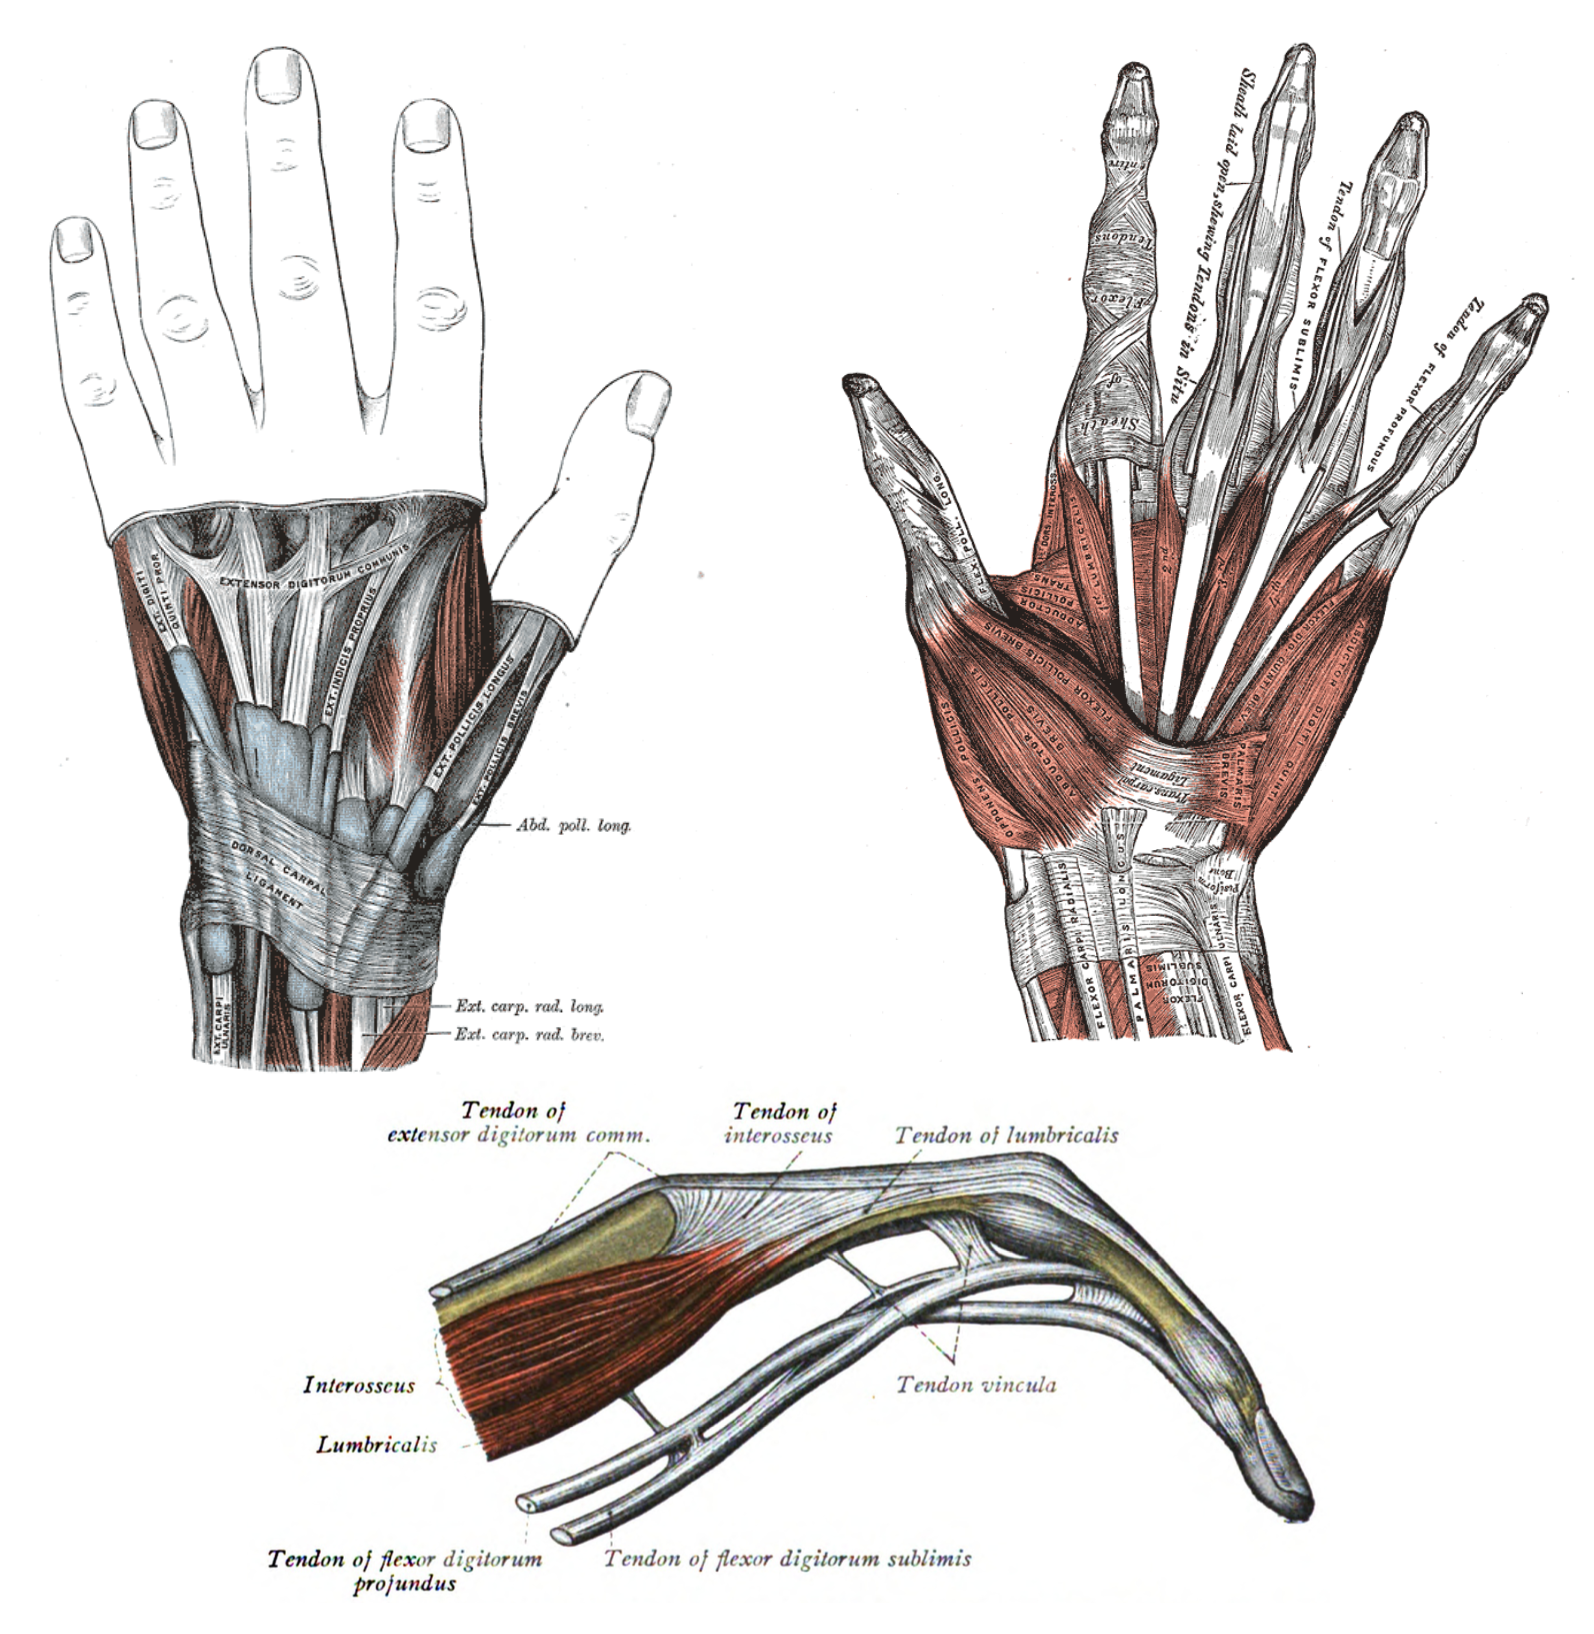
\includegraphics[width=0.7\linewidth]{files/EPpXta8zJdzN048lz8AR-198b50dfe4a0831985ee6ca2f0f5e8fd.png}
\caption[]{Tendons of the hand. Dorsal (top left) and palmar (top right) views. From Gray's Anatomy, via Wikimedia Commons, Public Domain. Bottom center: Drawing of a single finger, showing specific extensor and flexor tendons. Image credit: Sobotta's Atlas and Text-book of Human Anatomy 1909, via Wikimedia Commons, Public Domain.}
\label{cLezcHezN0}
\end{figure}

\subsection{Study questions}

\begin{enumerate}
\item On which side of the prosthetic hand do you need to place the threads if you want them to

act as finger flexor/extensor tendons?


\item Where should you fix the threads if you want them to flex/extend the MCP, PIP, or DIP joints?


\item Will you be able to accomplish individual control of the fingers and their different joints? If

not, why? If so, how?
\end{enumerate}

\section{Experimental procedure}

\subsection{Construct the lightweight model hand}

\begin{enumerate}
\item On a 20 x 30 cm rectangular piece of cardboard or other lightweight material, trace your hand and a portion of the wrist and forearm with a pencil or pen
\item Using the traced shaped as a guide, cut out the cardboard hand, and label one side 'dorsal' and the other side 'palmar'. Save the extra cardboard for later steps
\item On the palmar side, draw horizontal lines on the fingers where the major MCP, DIP, and IP joints would be
\item Take the five pieces of thread (each approx. 30 cm length), and tape or glue one end of each thread to each of the distal fingertips
\item Once each thread is fixed at the tip, run the threads down each corresponding finger on the palmar as if they were large, single tendons and staple (or otherwise fix) the threads where each joint is marked
\item An additional staple may be necessary further down the palm to better fix each thread
\item Depending on the consistency of the cardboard, the hand may need reinforcement in key places. If so, use the remaining cardboard and cut rectangular strips slightly less than the width and length of each finger and a larger rectangle about the size of the palm. Glue these to the dorsal side of the hand
\end{enumerate}

\subsection{Connect the motor}

\begin{enumerate}
\item At the base of the cardboard forearm, cut a rectangular hole with the dimensions of the servomotor MG995 (approximately 20 x 40mm for that model, but exact size may vary)
\item Insert the servomotor into the hole in the model hand, and fix it in place using the silicon glue and gun
\item Run the loose end of each thread down to the base of the hand and connect them to propeller on the servomotor. Leave some but not too much slack in the threads, and readjust as needed
\item Connect the cables on the servomotor to the Muscle SpikerShield, following the color code on the board
\end{enumerate}

\begin{figure}[!htbp]
\centering
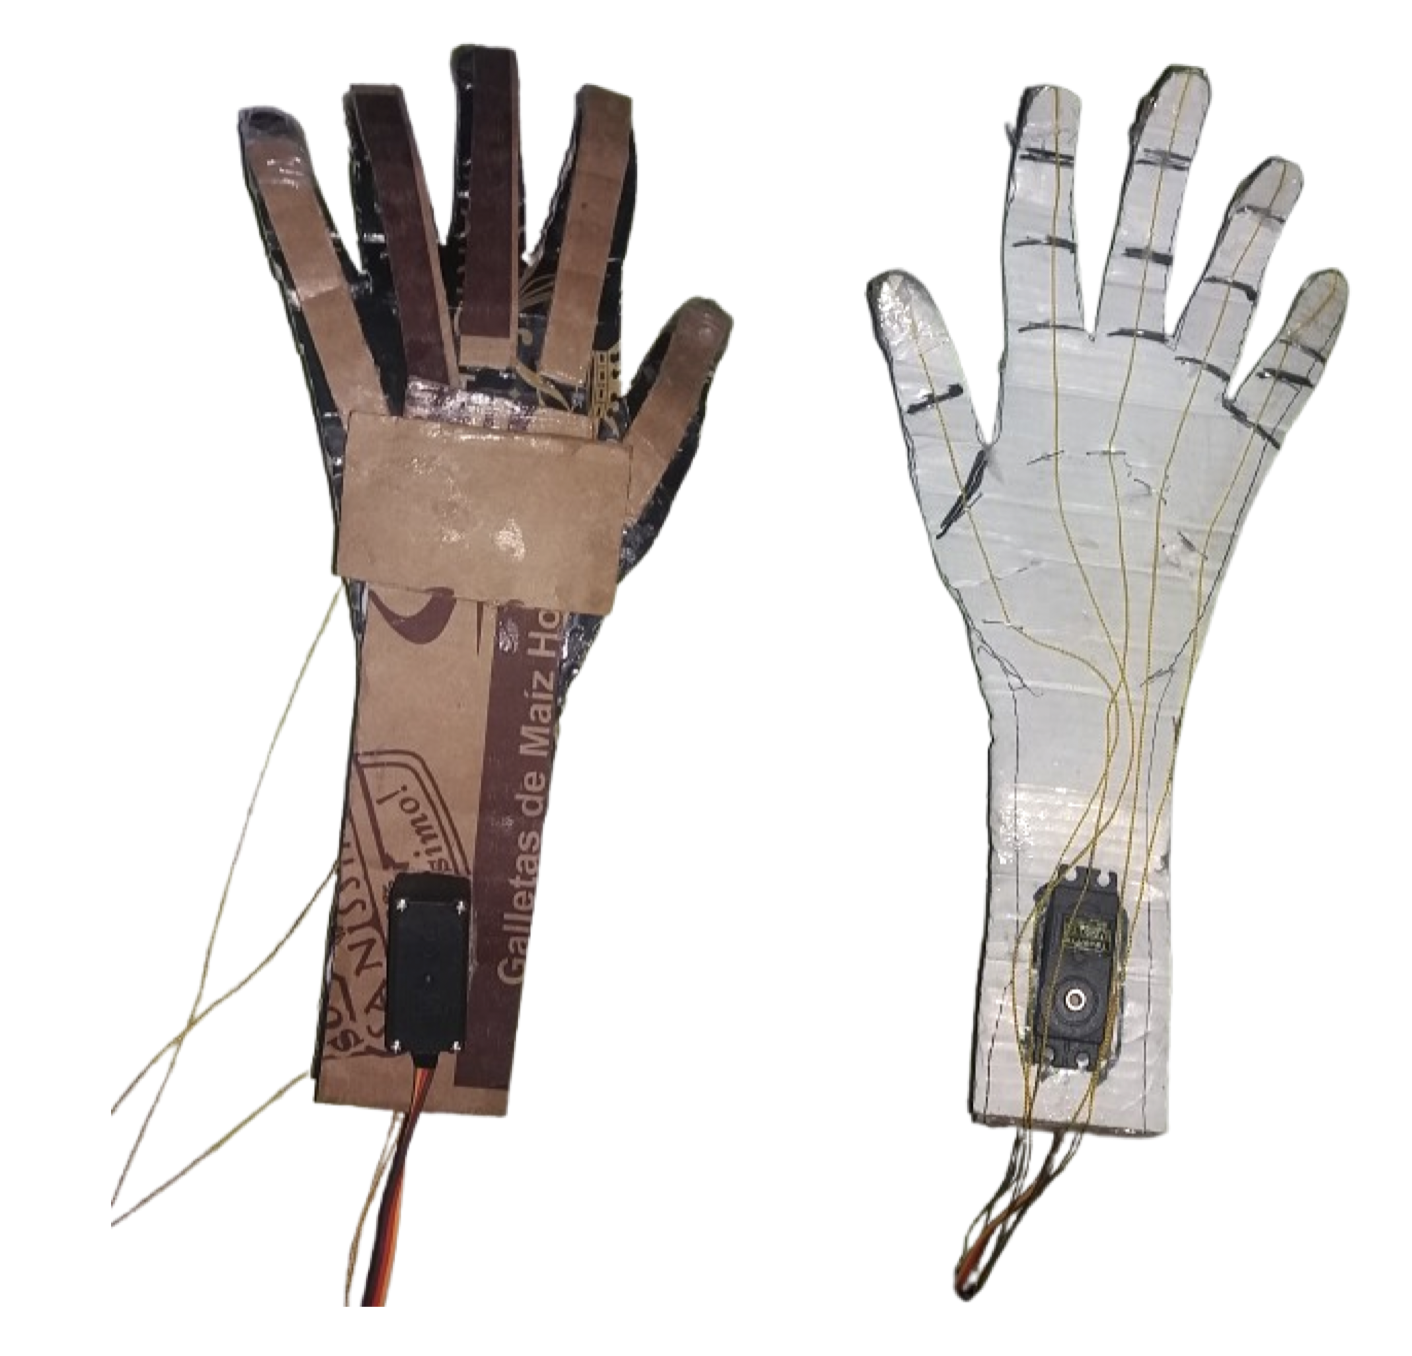
\includegraphics[width=0.7\linewidth]{files/EPpXta8zJdzN048lz8AR-4f049cefc47709553d6ee28b9743dba5.png}
\caption[]{Cardboard model hand, showing the dorsal (left) and palmar (right) sides. Yellow threads represent tendons that run down each finger to the black rectangular servomotor at the base. Image credit: Daniel Gómez Pérez}
\label{mlSs5a3cGd}
\end{figure}

\subsection{Program the Arduino}

\begin{enumerate}
\item Connect the Muscle SpikerShield to your computer using the blue USB cable provided
\item Open the Arduino software (free downloads at \href{https://docs.arduino.cc/software}{https://docs.arduino.cc/software})
\item From the `Tools' menu, select the board `Arduino Uno' and the port in which the device is connected to the your computer
\item In the program terminal, write the code that will be used to configure the interface and allow it to transmit electrical signals generated in the muscle to move the servomotor. Full code is provided by Backyard Brains at \href{https://docs.backyardbrains.com/retired/experiments/MuscleSpikerShield\_GripperHand}{https://docs.backyardbrains.com/retired/experiments/MuscleSpikerShield\_GripperHand}
\item Once the code is written, compile and upload it to the Arduino board
\end{enumerate}

\subsection{Set up EMG recording and interface}

\begin{enumerate}
\item Place two round surface electrodes over the biceps muscle, a few centimeters apart and aligned in parallel with the muscle fibers
\item Hold the black alligator clip (reference) in your hand, or connect it to another surface electrode on the back of your hand or wrist
\item Connect each of the red alligator clips on the end of the orange cable to one of the muscle surface electrodes. Make sure the metal clips do not touch and try to avoid entangling the cables
\item If necessary, the EMG recording can be quickly tested using the Muscle SpikerBox and a smartphone (see \href{https://curvenote.com/oxa:EPpXta8zJdzN048lz8AR/hZTnTYzQR5EQmCKX51Wj}{Ch. 1: Muscle physiology and EMG basics})
\item Plug the orange cable into its port on the SpikerShield
\item Connect one 9V battery to the board using its adapter in the black connector, and connect another battery to the Arduino
\end{enumerate}

\subsection{Contractions and model hand movement}

\begin{enumerate}
\item The volunteer can begin performing bicep contractions
\item The servomotor should move with each contraction, with the extent of its movement depend on the strength of the EMG signal, i.e. the force exerted.
\item Try perform contractions of varying intensity and observe which LEDs light up and how much movement is achieved in the model hand.
\end{enumerate}

\textbf{Next steps:} Think about how you would re-design the hand to have both flexors and extensors (this model has only flexors and extension is passive). Think about other ways you could improve the design, see for example this model from Backyard Brains \href{https://docs.backyardbrains.com/retired/experiments/diyneuroprosthetic}{https://docs.backyardbrains.com/retired/experiments/diyneuroprosthetic}. Or, if you have access to a 3D printer, here's another interesting design \href{https://www.instructables.com/Servo-Controlled-Prosthetic-Hand/}{https://www.instructables.com/Servo-Controlled-Prosthetic-Hand/}.

\clearpage
\bibliography{main.bib}

\end{document}
